\chapter{Eksperymentalny algorytm klasyfikatora fingerprintów}

\section{Motywacja}
Wcześniej w niniejszej pracy zostało zaznaczone, że \emph{fingerprint} może być
bardziej unikalny kosztem jego stabilności i odwrotnie. Aby zgrupować kolejne
\emph{fingerprinty} tej samej przeglądarki internetowej, których różnice
wynikają z naturalnych przemian tej przeglądarki (np. aktualizacja), możemy użyć
klasyfikatora opartego na odpowiednim algorytmie. Tę relację przedstawia Rys. 7.
Dzięki takiemu rozwiązaniu jesteśmy w stanie zachować wiarygodny wskaźnik
entropii, używając średnio bardziej unikalnych \emph{fingerprintów} o mniejszej
stabilności.

Podobne (choć bardziej ograniczone) rozwiązanie zastosował Eckersley w swojej
pracy, w której po raz pierwszy opisał \emph{fingerprinting} przeglądarek
internetowych \cite[s. 13]{eckersley2010unique}.

\begin{figure}
	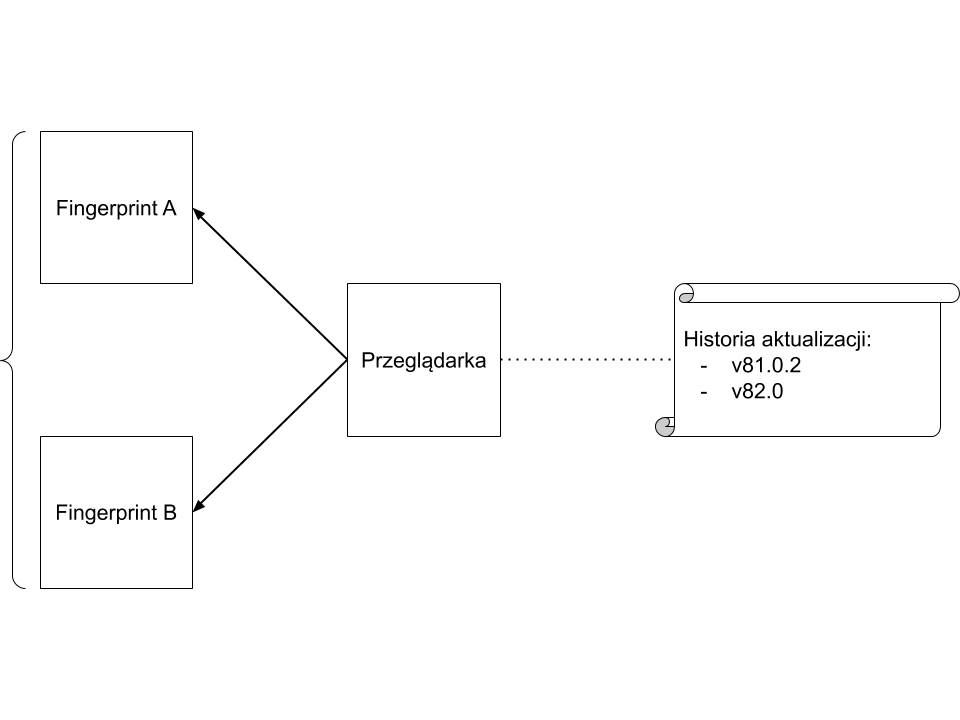
\includegraphics[width=\textwidth,keepaspectratio]{img/09}
	\source{Diagram przygotowany przez autora niniejszej pracy}
	\caption{Relacja \emph{fingerprint}--przeglądarka}
\end{figure}

\section{Opis algorytmu}
Aby zgrupować kolejne, podobne do siebie \emph{fingerprinty} należy wyznaczyć
podobieństwo każdego nowego \emph{fingerprintu} do wszystkich przechowywanych i
utożsamić go z tym, do którego jest najbardziej podobny (powyżej pewnej wartości
podobieństwa). Można to zrobić na parę sposobów. Jednym z najsensowniejszych
rozwiązań wydaje się podejście, w którym określa się podobieństwo cech
(komponentów) \emph{fingerprintu}, pomiędzy którymi istnieje relacja większości
(częściowy porządek). Tak można porównywać na przykład nagłówki User-Agent
(zawiera w sobie wersję oprogramowania) jako komponent dwóch porównywanych
\emph{fingerprintów}. Z tych porównań można wnioskować o ogólnym podobieństwie
dwóch \emph{fingerprintów}.

Porównywanie podobieństwa komponentów, które bezpośrednio lub pośrednio wynikają
z np. parametrów sprzętowych urządzenia (na przykład \emph{fingerprint} elementu
\texttt{canvas}), wydaje się bezcelowe. Ich wartość zwykle nie ulega zmianie i
należałoby zastanowić się nad istnieniem częściowego porządku w ich zbiorze.
Jednakże ich pewna niezmienność i dalej porównywanie tych komponentów na
zasadzie równoważności może być przydatne, w szacowaniu jak bardzo ogólne
podobieństwo jest wiarygodne.

Metryką określającą podobieństwo do siebie dwóch komponentów będzie odległość
Levenshteina, która jest powszechnie stosowaną miarą odmienności skończonych
ciągów znaków.

\subsection{Odległość Levenshteina}
Odległość Levenshteina nie jest na tyle popularnym algorytmem, aby znalazł on
swoją implementację w bibliotekach standardowych większości popularnych języków
oprogramowania. Z tego względu autor niniejszej pracy zdecydował się na
własnoręczną implementację.

\subsubsection{Definicja}
Odległość Levenshteina pomiędzy dwoma łańcuchami znaków \(a\) i \(b\) o
długościach odpowiednio \(i\) i \(j\), zdefiniowana jest jako
\begin{displaymath}
	\operatorname{ol}(i,j)=
	\begin{cases}
		\max(i,j)                    & \text{jeśli }\min(i,j)=0,  \\
		\min
		\begin{cases}
		\operatorname{ol}(i-1,j)+1 \\
		\operatorname{ol}(i,j-1)+1 \\
		\operatorname{ol}(i-1,j-1)   & \text{jeśli }a_i=b_j,      \\
		\operatorname{ol}(i-1,j-1)+1 & \text{jeśli }a_i \neq b_j. 
	\end{cases} & \text{w innym przypadku}.
	\end{cases}
\end{displaymath}

\subsubsection{Algorytm Wagnera--Fischera}
Bezpośrednia implementacja (z definicji) odległości Levenshteina ma zasadniczy
problem: tak zaimplementowany algorytm będzie działać w czasie
ponadwielomianowym. Aby się o tym przekonać, wystarczy narysować drzewo wywołań
rekurencyjnych i zauważyć, że kolejne wywołania nie są rozłączne (nie jest to
oczywiście formalny dowód). Odległość Levenshteina cechuje własność optymalnej
podstruktury i bazując na programowaniu dynamicznym, można znaleźć algorytm
działający w czasie wielomianowym.

Jednym z takich algorytmów jest algorytm Wagnera--Fischera\footnote{Algorytm
	miał wielu wynalazców. Nazwa ,,Wagnera--Fischera'' powinna być traktowana
	jedynie jako zwyczajowa:
	https://en.wikipedia.org/wiki/Wagner-Fischer\_algorithm\#History} (Algorytm 2)
\cite{wagner1974string}. Implementacja 4 przedstawia implementację algorytmu
Wagnera--Fischera. Implementacja 5 jest optymalnym wariantem tego algorytmu
(biorąc pod uwagę zużycie pamięci; Implementacja 4 zużywa kwadratową ilość
pamięci a Implementacja 5 liniową). Taki wariant jest stosowany później w
algorytmie klasyfikatora.

% TODO It should be more consistent with the style in the others.
\begin{algorithm}
	\SetAlgoVlined
	\SetAlgoCaptionSeparator{.}
	\SetKwInOut{Input}{Dane}
	\SetKwInOut{Output}{Wynik}
	\SetKwData{VarA}{a}
	\SetKwData{VarB}{b}
	\SetKwData{VarM}{m}
	\SetKwData{VarN}{n}
	\SetKwFunction{Minimum}{minimum}
	\BlankLine
	\Input{ciągi znaków \VarA i \VarB o długościach odpowiednio \VarM i \VarN}
	\Output{odległość Levenshteina}
	\BlankLine
	$d \leftarrow [0 \dots m, 0 \dots n]$
	\BlankLine
	\For{$i \leftarrow 1$ \KwTo \VarM}{
		$d[i, 0] \leftarrow i$
	}
	\For{$j \leftarrow 1$ \KwTo \VarN}{
		$d[0, j] \leftarrow j$
	}
	\For{$j \leftarrow 1$ \KwTo \VarN}{
		\For{$i \leftarrow 1$ \KwTo \VarM}{
			\eIf{$a[i - 1] = b[j - 1]$}{
				$c \leftarrow 0$
				}{
				$c \leftarrow 1$
			}
			$d \leftarrow$ \Minimum{$d[i - 1, j] + 1, d[i, j - 1] + 1, d[i - 1, j - 1] + c$}
		}
	}
	\Return{$d[m, n]$}
	\caption{Algorytm Wagnera--Fischera}
\end{algorithm}

\lstinputlisting[float,language=Go,caption=Algorytm Wagnera--Fischera w Go,firstline=18,lastline=44,tabsize=4]{go/levenshtein.go}

\lstinputlisting[float,language=Go,caption=Algorytm Wagnera--Fischera w Go (liniowa pamięć),firstline=46,lastline=74,tabsize=4]{go/levenshtein.go}

\section{Pseudokod}
Algorytm 3 przedstawia eksperymentalny algorytm klasyfikatora.

\begin{algorithm}
	\SetAlgoVlined
	\SetAlgoCaptionSeparator{.}
	\SetKwInOut{Input}{Dane}
	\SetKwInOut{Output}{Wynik}
	\BlankLine
	\Input{\emph{fingerprint}}
	\Output{\emph{fingerprint}, do którego jest najbardziej podobny, jeśli istnieje}
	\BlankLine
	\caption{Eksperymentalny klasyfikator}
\end{algorithm}

\section{Ocena złożoności czasowej i pamięciowej}

\section{Ocena efektywności}
